\documentclass[10pt]{standalone}
\usepackage{commands}

\begin{document}
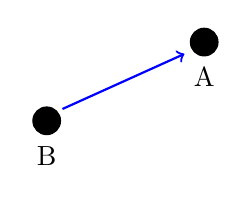
\begin{tikzpicture}
    \draw[blue, thick, ->] (0.2, 0.15) -- (1.75, 0.85);
    \draw[fill=black] (0, 0) circle (5pt);
    \node[below] at (0, -0.2) {B};
    \draw[fill=black] (2, 1) circle (5pt);
    \node[below] at (2, 0.8) {A};
\end{tikzpicture}
\end{document}